% Kiara DB -- manuscript prepared for IEEE Access.
%
% Submission build: place the official IEEE Access template files
% (ieeeaccess.cls, spotcolor.sty, logo.png, notaglinelogo.png, bullet.png and
% the template fonts) next to this file. When ieeeaccess.cls is present it is
% used automatically; otherwise the manuscript falls back to IEEEtran so the
% content can be proofread with any standard TeX distribution.
\IfFileExists{ieeeaccess.cls}{%
  \documentclass{ieeeaccess}\newif\ifaccess\accesstrue
}{%
  \documentclass[journal]{IEEEtran}\newif\ifaccess\accessfalse
}

\usepackage{cite}
\usepackage{amsmath,amssymb,amsfonts}
\usepackage{algorithm}
\usepackage[noend]{algpseudocode}
\usepackage{graphicx}
\usepackage{textcomp}
\usepackage{array}
\newcolumntype{P}[1]{>{\raggedright\arraybackslash}p{#1}}
\usepackage{booktabs}
\usepackage{multirow}
\usepackage{url}
\usepackage{xcolor}
\usepackage{tikz}
\usetikzlibrary{arrows.meta,positioning,shapes.misc,fit}
\usepackage{pgfplots}
\pgfplotsset{compat=1.18}

\ifaccess\else
  % Times-compatible text and math fonts for the IEEEtran proof build.
  \usepackage[T1]{fontenc}
  \usepackage{newtxtext}
  \usepackage{newtxmath}
  % Minimal shims for the IEEE Access front-matter macros.
  \newcommand{\history}[1]{}
  \newcommand{\doi}[1]{}
  \newcommand{\tfootnote}[1]{}
  \newcommand{\corresp}[1]{}
  \newcommand{\headeretal}{et al.}
  \newcommand{\EOD}{}
  \newskip\titlepgskip
\fi

\newtheorem{definition}{Definition}
\newtheorem{lemma}{Lemma}
\newtheorem{theorem}{Theorem}
\newtheorem{proposition}{Proposition}

\newcommand{\kiara}{Kiara}
\newcommand{\op}[1]{\texttt{\small #1}}
\newcommand{\pre}{\mathrm{pre}}
\newcommand{\post}{\mathrm{post}}
\newcommand{\lev}{\mathrm{lev}}
\renewcommand{\algorithmicrequire}{\textbf{Input:}}
\renewcommand{\algorithmicensure}{\textbf{Output:}}

\newcommand{\PaperTitle}{Kiara DB: Composite-Index-Free Multi-Attribute Retrieval over Read-Mostly In-Memory Data with Depth-First-Numbered Attribute Tries}

\newcommand{\PaperAbstract}{%
Applications that serve read-mostly reference data, such as product catalogs, schedules, configuration rules, and inventories, must answer conjunctive queries over attribute subsets that users choose at run time. A composite index serves only the combinations that match its key prefix: covering every equality combination of $m$ attributes requires $\binom{m}{\lfloor m/2\rfloor}$ B-tree orderings, for example 252 for ten attributes. Kiara DB avoids composite indexes by storing records as root-to-leaf paths in an attribute-ordered trie, numbering nodes by depth-first traversal, and indexing each trie level separately; a conjunction then reduces to interval-containment joins between sorted posting lists. This paper extends our 2020 description of equality search to the complete system: typed scalar, temporal, and collection predicates; prefix-partitioned interval trees for stored ranges; eleven operators, including negation; an adaptive two-direction structural join over disjunctive posting-list collections; and a text layer with stemming, one-edit correction, prefix prediction, and coverage-maximizing cross-field keyword search. We evaluate Kiara 2.0.16 against Apache Lucene and against tuned and generic-index configurations of SQLite and VoltDB Community Edition, using an independent result oracle and repeated fresh-process trials comprising 1.04 million timing observations. On equivalent structured queries, Lucene's aggregate latency was 3.5--16.1 times Kiara's, and Kiara had lower aggregate latency than generic-index SQL configurations on most datasets, particularly for collection membership. Tuned SQL engines were faster for wide scalar conjunctions, broad windows, and some exclusions, and Kiara's 100{,}000-record builds were 26--38$\times$ slower than Lucene's. A cost model traces these outcomes to specific design choices and identifies concrete remedies.}

\newcommand{\PaperKeywords}{Composite index, in-memory database, inverted index, interval encoding, multi-attribute search, read-mostly data, structural join, trie, type-ahead search, spelling correction, database benchmarking.}

\begin{document}

\history{Date of publication xxxx 00, 0000, date of current version xxxx 00, 0000.}
\doi{10.1109/ACCESS.0000.DOI}

\title{\PaperTitle}

\ifaccess
  \author{\uppercase{Anuj Kapoor}\authorrefmark{1}}
  \address[1]{Kapoor Labs, USA (e-mail: anuj.kapoor@kapoorlabs.com)}
  \tfootnote{This work received no external funding.}
  \markboth{A. Kapoor: Composite-Index-Free Multi-Attribute Retrieval with Kiara DB}{A. Kapoor: Composite-Index-Free Multi-Attribute Retrieval with Kiara DB}
  \corresp{Corresponding author: Anuj Kapoor (e-mail: anuj.kapoor@kapoorlabs.com).}
  \begin{abstract}\PaperAbstract\end{abstract}
  \begin{keywords}\PaperKeywords\end{keywords}
  \titlepgskip=-21pt
  \maketitle
\else
  \author{Anuj~Kapoor%
    \thanks{A. Kapoor is with Kapoor Labs, USA (e-mail: anuj.kapoor@kapoorlabs.com).}%
    \thanks{This work received no external funding.}}
  \markboth{IEEE Access (manuscript in preparation)}{Kapoor: Composite-Index-Free Multi-Attribute Retrieval with Kiara DB}
  \maketitle
  \begin{abstract}\PaperAbstract\end{abstract}
  \begin{IEEEkeywords}\PaperKeywords\end{IEEEkeywords}
\fi

\section{Introduction}
\label{sec:introduction}

\IEEEPARstart{M}{any} applications keep a moderately sized, read-mostly dataset in memory and query it far more often than they change it. Examples include product catalogs behind faceted storefronts, flight and event schedules, pricing and configuration rules, and parts inventories. Their queries share a distinctive shape. Each query is a conjunction of predicates, but \emph{which} attributes participate is chosen at run time by a user interface, a rules engine, or a calling service. A shopper may filter by brand and size; the next request may filter by region, price band, and an included date. The set of attribute combinations that must be fast is therefore open-ended.

Conventional physical designs handle this poorly. A hash index serves exactly one attribute set. A composite B-tree~\cite{bayer1972organization,comer1979ubiquitous} serves the attribute sets that form a prefix of its key order. Index advisors~\cite{chaudhuri1997efficient,valentin2000db2} select a small set of such indexes for a \emph{known} workload, but an unpredictable workload defeats them by construction. Covering every equality combination with prefix seeks requires $\binom{m}{\lfloor m/2\rfloor}$ distinct key orders for $m$ attributes (Proposition~\ref{prop:indexcount}), which is 252 orders for ten attributes and 184{,}756 for twenty. Engines instead fall back to single-attribute indexes combined by row-identifier intersection~\cite{oneil1997improved,lemire2016roaring}, to inverted-index engines such as Lucene~\cite{mccandless2010lucene}, or to scanning.

Our 2020 article~\cite{kapoor2020efficient} proposed a different organization for static in-memory data, later released as the open-source Java library \emph{Kiara DB}~\cite{kiara2026software}. Records are inserted as root-to-leaf paths in a trie whose levels correspond to attributes. A depth-first traversal assigns each node an interval of visit numbers, so that ancestry becomes interval containment. Each level receives one hash index from values to posting lists of trie nodes, and a conjunction over any subset of attributes is answered by joining those posting lists through interval containment. Only $m$ logical indexes are needed, regardless of which combinations are queried.

That article described equality conjunctions and a worst-case bound. It left four questions open, which this paper answers:
\begin{enumerate}
\item How does the model extend beyond equality to ordered comparisons, temporal values, multi-valued attributes, stored intervals, missing values, and negation, while keeping one logical index per attribute?
\item Can the same structures support the text-oriented access patterns that interactive applications need, such as typo tolerance, stemming, type-ahead, and keyword queries whose target attributes are unknown?
\item Which query shapes does the design favor or penalize, and why?
\item How does a faithful implementation compare with mature engines under careful, correctness-checked measurement?
\end{enumerate}

\subsection{Contributions}
\begin{itemize}
\item \textbf{Formal model and a corrected bound.} We formalize the attribute trie, prove correctness of level-wise reduction, and show that the minimum number of composite B-tree orders covering all equality subsets as prefixes is $\binom{m}{\lfloor m/2\rfloor}$, correcting the count reported in~\cite{kapoor2020efficient} (Section~\ref{sec:model}).
\item \textbf{A typed, multi-valued, interval-aware extension.} We describe how Kiara indexes numeric, temporal, enumerated, Boolean, case-folded, collection-valued, and interval-valued attributes; its eleven operators; prefix-partitioned augmented interval trees; and an adaptive, two-direction structural join over \emph{disjunctive posting-list collections} (Section~\ref{sec:system}).
\item \textbf{An integrated text layer.} We describe index-time and query-time Snowball stemming, one-edit correction over a character trie, breadth-first prefix prediction, and a coverage-maximizing keyword search that discovers which attributes each keyword binds to and composes the result with hard structured filters (Section~\ref{sec:text}).
\item \textbf{A cost model.} We derive per-operator candidate fan-out and reduction costs, and the build cost of trie insertion. The model explains both Kiara's largest wins and its largest losses in our experiments (Section~\ref{sec:cost}).
\item \textbf{A transparent multi-engine evaluation.} Seven benchmark suites compare Kiara~2.0.16 with Apache Lucene~10.5.2, SQLite~3.53.4, and VoltDB Community Edition~10.1.1. SQLite and VoltDB are evaluated in expert-tuned and generic-index configurations, and VoltDB also in a client--server configuration. Every timed result is validated against an independent scan oracle. Semantic mismatches are reported, not hidden (Sections~\ref{sec:methodology}--\ref{sec:results}).
\end{itemize}

The rest of the paper is organized as follows. Section~\ref{sec:related} reviews related work. Section~\ref{sec:model} formalizes the model. Section~\ref{sec:system} presents the system and Section~\ref{sec:cost} its cost model. Sections~\ref{sec:methodology} and~\ref{sec:results} describe the evaluation. Section~\ref{sec:discussion} discusses implications, threats to validity, limitations, and future work, and concludes the paper.

\section{Related Work}
\label{sec:related}

\subsection{Composite Indexes and Physical Design}
B-trees~\cite{bayer1972organization,comer1979ubiquitous,graefe2011modern} remain the default ordered index in relational systems. A composite B-tree on $(a_1,\dots,a_k)$ supports an equality seek on any prefix $\{a_1,\dots,a_j\}$. Other conjunctions need a partial seek followed by residual filtering, or a different index. Automated physical-design tools such as AutoAdmin~\cite{chaudhuri1997efficient} and the DB2 Advisor~\cite{valentin2000db2} choose indexes that minimize the estimated cost of a given workload under a storage budget. Adaptive approaches such as database cracking~\cite{idreos2007cracking} reorganize data incrementally as queries arrive. All of these approaches optimize for queries that have been observed or predicted. Kiara instead targets workloads in which the attribute combination is an unconstrained user choice. It provides the same logical access path for every combination without a workload model.

\subsection{Index Intersection, Bitmaps, and Inverted Lists}
The standard alternative to composite indexes is to keep one index per attribute and intersect their row-identifier lists or bitmaps. Variant and bitmap indexes~\cite{oneil1997improved}, compressed bitmaps such as Roaring~\cite{lemire2016roaring}, and the sorted posting lists of inverted files~\cite{zobel2006inverted} all follow this pattern. Efficient intersection of sorted lists has been studied extensively. Adaptive algorithms~\cite{demaine2000adaptive} and probing of the larger list from the smaller~\cite{baezayates2004fast} make cost depend on list sizes rather than on collection size. SIMD techniques further accelerate intersection~\cite{lemire2016simd}. Kiara's per-level posting lists are also sorted. However, they contain \emph{trie nodes} rather than record identifiers, and the lists for different attributes reside at different depths. Their join is therefore a containment join rather than an identity intersection. Prefix sharing lets a single node in a shallow list stand for many records.

\subsection{Interval Encodings and Structural Joins}
Labeling tree nodes with preorder and postorder numbers, so that ancestry reduces to interval containment, dates back to Dietz~\cite{dietz1982maintaining}. It was later used extensively for XML query processing. Zhang~\emph{et al.}~\cite{zhang2001supporting} evaluated containment queries in a relational engine, and Grust's XPath accelerator~\cite{grust2002accelerating} encoded document axes as regions of the pre/post plane. Al-Khalifa~\emph{et al.}~\cite{alkhalifa2002structural} introduced stack-based \emph{structural joins} between sorted ancestor and descendant lists. Bruno~\emph{et al.}~\cite{bruno2002holistic} generalized them to holistic twig joins. Kiara applies the same encoding to a different object: a trie built from relational records, in which every root-to-leaf path is a record and every query is a linear path pattern over a subset of levels. Its reduction step is a structural join specialized in two ways. First, it chooses between probing ancestors by binary search and enumerating contiguous descendant runs. Second, it operates on \emph{collections} of sorted lists rather than on a single merged list (Section~\ref{sec:reduction}).

\subsection{Main-Memory and Embedded Engines}
Main-memory database systems remove disk-oriented costs from query processing. H-Store~\cite{kallman2008hstore} and its commercial successor VoltDB~\cite{stonebraker2013voltdb} partition data and run precompiled stored procedures serially per partition. HyPer~\cite{kemper2011hyper} combines transactional and analytical processing in memory, and column stores~\cite{boncz2008breaking,abadi2008columnstores} optimize scans and aggregates. SQLite~\cite{gaffney2022sqlite} is the most widely deployed embedded SQL engine and supports private in-memory databases. Main-memory index structures include T-trees~\cite{lehman1986study} and adaptive radix trees~\cite{leis2013art}. Kiara is narrower than all of these. It is an embedded, read-mostly library without transactions, durability, or SQL. Its contribution is the logical organization of indexes for ad hoc conjunctions, which we compare against these engines' mature implementations.

\subsection{Text Search, Autocompletion, and Spelling}
Lucene~\cite{mccandless2010lucene} implements inverted indexes with numeric points, interval fields, analyzers, and BM25 relevance ranking~\cite{robertson2009bm25}. Stemming commonly uses Porter's algorithm~\cite{porter1980algorithm} or its Snowball successors~\cite{porter2001snowball}. Spelling correction is usually framed in terms of Damerau--Levenshtein distance~\cite{damerau1964technique,levenshtein1966binary}. Supporting index structures include BK-trees~\cite{burkhard1973approaches}, Levenshtein automata~\cite{schulz2002fast}, and the dictionary methods surveyed by Boytsov~\cite{boytsov2011indexing}. Autocompletion has been studied as prefix search over succinct indexes~\cite{bast2006type} and with error tolerance~\cite{ji2009efficient}. Keyword search over relational databases, including DISCOVER~\cite{hristidis2002discover}, DBXplorer~\cite{agrawal2002dbxplorer}, and BANKS~\cite{bhalotia2002banks}, finds tuples or joined tuple trees that contain user keywords without the user naming attributes. Kiara's best-match search addresses a single-relation version of that problem. It binds each keyword to the attributes whose indexes contain it and maximizes the number of keywords that one structured conjunction can satisfy. It deliberately omits term weighting.

\subsection{Benchmarking Methodology}
Database performance comparisons are notoriously sensitive to configuration, warm-up, and reporting choices~\cite{raasveldt2018fair}. Managed runtimes add just-in-time compilation and garbage-collection variance, which motivates repeated fresh-process trials and statistically rigorous summaries~\cite{georges2007statistically}. Ratios of execution times should be aggregated with a geometric mean~\cite{fleming1986how}. Resampling methods~\cite{efron1993introduction} can then express trial-to-trial uncertainty. Our methodology follows these recommendations and adds an engine-independent correctness oracle.

\section{The Attribute-Trie Model}
\label{sec:model}

This section formalizes the organization introduced in~\cite{kapoor2020efficient}, which all later extensions preserve.

\subsection{Records, Tries, and Interval Labels}

\begin{definition}[Store and attribute trie]
A \emph{store} has an ordered schema $A=(a_1,\dots,a_m)$ and a multiset of records $D$, where record $r$ assigns a normalized value $r[a_\ell]$ to each attribute. The \emph{attribute trie} $T(D)$ is the smallest rooted tree in which every record $r$ is spelled by a root-to-leaf path $\langle \rho, v_1,\dots,v_m\rangle$ with $\mathrm{val}(v_\ell)=r[a_\ell]$, and siblings carry distinct values. Node $v_\ell$ is at level $\lev(v_\ell)=\ell$.
\end{definition}

Level $\ell$ therefore stores each distinct value of $a_\ell$ once per distinct prefix $(r[a_1],\dots,r[a_{\ell-1}])$. Records that share a prefix share its nodes. This prefix sharing is the source of the deduplication discussed in~\cite{kapoor2020efficient}. Records that agree on every attribute collapse into one path. Kiara presents such records once, so applications that need multiset semantics include a distinguishing attribute.

After loading, one depth-first traversal assigns each node two numbers from a single counter $c$. The counter is incremented when the traversal enters a node and again when it leaves it:
\begin{equation}
\pre(v) = c_{\mathrm{enter}}(v), \qquad \post(v) = c_{\mathrm{leave}}(v).
\end{equation}
Fig.~\ref{fig:trie} shows an example.

\begin{figure}[t]
\centering
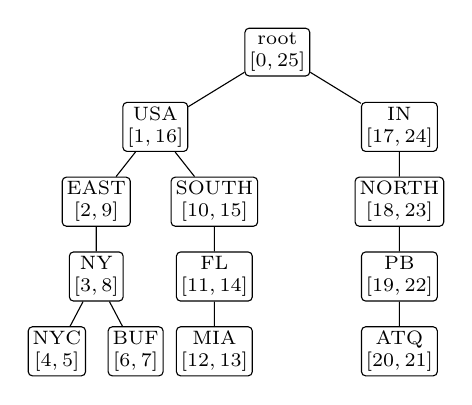
\begin{tikzpicture}[
  level distance=9.5mm,
  every node/.style={draw, rounded corners=1.5pt, font=\scriptsize, inner sep=1.6pt, align=center, fill=white},
  level 1/.style={sibling distance=31mm},
  level 2/.style={sibling distance=15mm},
  level 3/.style={sibling distance=11mm},
  level 4/.style={sibling distance=10mm},
  edge from parent/.style={draw, -}]
\node {root\\$[0,25]$}
  child {node {USA\\$[1,16]$}
    child {node {EAST\\$[2,9]$}
      child {node {NY\\$[3,8]$}
        child {node {NYC\\$[4,5]$}}
        child {node {BUF\\$[6,7]$}}}}
    child {node {SOUTH\\$[10,15]$}
      child {node {FL\\$[11,14]$}
        child {node {MIA\\$[12,13]$}}}}}
  child {node {IN\\$[17,24]$}
    child {node {NORTH\\$[18,23]$}
      child {node {PB\\$[19,22]$}
        child {node {ATQ\\$[20,21]$}}}}};
\end{tikzpicture}
\caption{Attribute trie for four records with schema (Country, Region, State, City). Each node is labeled with $[\pre,\post]$. The level-2 posting list for \texttt{EAST} is $\langle[2,9]\rangle$ and the level-4 list for every city holds one node. The query Region$=$EAST $\wedge$ City$=$BUF reduces to testing whether $[6,7]\subset[2,9]$.}
\label{fig:trie}
\end{figure}

\begin{lemma}[Ancestry as containment]
\label{lem:ancestry}
Node $u$ is a proper ancestor of $v$ if and only if $\pre(u)<\pre(v)$ and $\post(v)<\post(u)$.
\end{lemma}
\begin{IEEEproof}
This is the parenthesis property of depth-first search~\cite{cormen2009introduction}. The traversal enters $v$ after entering $u$ and leaves $v$ before leaving $u$ exactly when $v$ lies in the subtree of $u$.
\end{IEEEproof}

\begin{lemma}[Order within a level]
\label{lem:levelorder}
The intervals of distinct nodes at the same level are disjoint. Hence, ordering same-level nodes by $\pre$ is the same as ordering them by $\post$. Moreover, for any node $u$ with $\lev(u)<\ell$, the level-$\ell$ descendants of $u$ form a contiguous run in the $\pre$-ordered sequence of level-$\ell$ nodes.
\end{lemma}
\begin{IEEEproof}
Two same-level nodes are not ancestors of each other, so by the parenthesis property their intervals are disjoint, and disjoint intervals are ordered identically by either endpoint. The descendants of $u$ are exactly the nodes whose intervals lie inside $[\pre(u),\post(u)]$. Among pairwise disjoint intervals sorted by left endpoint, these occupy a contiguous range.
\end{IEEEproof}

\subsection{Level Indexes}
For each searchable level $\ell$, a hash index $I_\ell$ maps every key $k$ to a posting list $P_\ell(k)$ of level-$\ell$ nodes whose value yields key $k$. Kiara appends a node to its lists when the traversal \emph{leaves} the node. By Lemma~\ref{lem:levelorder}, every posting list is therefore sorted by $\pre$ without an explicit sort. This is the property that makes binary-search reduction possible~\cite{kapoor2020efficient}. In the 2020 design each node contributed one key. Section~\ref{sec:system} relaxes this so that a node contributes one key per element of a collection value, and adds ordered and interval structures over the key space of a level.

\subsection{Conjunctive Queries and Level-Wise Reduction}
A query $Q$ is a set of predicates, each constraining one attribute. For a constrained level $\ell$, let $C_\ell$ be the set of level-$\ell$ nodes whose values satisfy every predicate on $a_\ell$. Let $\ell_1<\dots<\ell_t$ be the constrained levels, and define
\begin{align}
R_1 &= C_{\ell_1}, \nonumber\\
R_i &= \{\, v\in C_{\ell_i} \;:\; \exists\, u\in R_{i-1},\ u \text{ is an ancestor of } v \,\}. \label{eq:reduction}
\end{align}

\begin{theorem}[Correctness of reduction]
\label{thm:reduction}
A record satisfies $Q$ if and only if its path passes through a node of $R_t$. The answer to $Q$ is the set of records spelled by root-to-leaf paths through $R_t$.
\end{theorem}
\begin{IEEEproof}
By induction on $i$, node $v$ at level $\ell_i$ belongs to $R_i$ exactly when the path from the root to $v$ passes through a node of $C_{\ell_j}$ for every $j\le i$. The base case is the definition of $R_1$. For the inductive step, each node has exactly one ancestor at level $\ell_{i-1}$, so the existential condition in~\eqref{eq:reduction} tests that unique ancestor. A record's path passes through its own value at every level. Therefore the record satisfies all predicates if and only if its node at level $\ell_t$ lies in $R_t$.
\end{IEEEproof}

Theorem~\ref{thm:reduction} holds for \emph{any} subset of constrained attributes. Once $R_t$ is known, its records are produced by walking parent pointers upward for attributes above $\ell_t$ and enumerating the subtree below each node of $R_t$ for attributes below it. By Lemma~\ref{lem:ancestry}, each ancestor test in~\eqref{eq:reduction} costs two integer comparisons. By Lemma~\ref{lem:levelorder}, a search over a sorted list either finds the unique candidate ancestor or delimits the contiguous run of candidate descendants.

\subsection{How Many Composite Indexes Would Be Needed?}
\label{sec:indexcount}

The motivation for the model is the number of composite indexes it avoids. We say a composite B-tree with key order $\pi=(\pi_1,\dots,\pi_k)$ \emph{serves} an attribute set $S$ by a full prefix seek if $S=\{\pi_1,\dots,\pi_{|S|}\}$.

\begin{proposition}
\label{prop:indexcount}
The minimum number of key orders that serve every nonempty $S\subseteq A$ by a full prefix seek is $\binom{m}{\lfloor m/2\rfloor}$.
\end{proposition}
\begin{IEEEproof}
The prefix sets of a key order form a chain in the Boolean lattice $2^A$. Serving every subset therefore requires a family of chains that covers the lattice. The subsets of size $\lfloor m/2\rfloor$ form an antichain of size $\binom{m}{\lfloor m/2\rfloor}$, and no chain contains two of them, which gives the lower bound~\cite{sperner1928satz,dilworth1950decomposition}. For the upper bound, the lattice admits a symmetric chain decomposition into exactly $\binom{m}{\lfloor m/2\rfloor}$ saturated chains $T_0\subset T_1\subset\dots\subset T_r$ with $|T_{i+1}\setminus T_i|=1$~\cite{debruijn1951set}. Each chain is realized by one key order that lists the elements of $T_0$ in any order, followed by the element added at each step. Every set in the chain is then a prefix set of that order.
\end{IEEEproof}

Table~\ref{tab:indexcount} compares this bound with the $2^m-1$ hash indexes needed for exact-match lookups on every subset and with the $m$ level indexes of the attribute trie. The 2020 article~\cite{kapoor2020efficient} reported $1+\sum_{k=1}^{m-1}k$ B-tree indexes, for example 46 for $m=10$. By Proposition~\ref{prop:indexcount} that count is below the lower bound of 252, so it cannot suffice. The corrected bound strengthens the original motivation. In practice, optimizers relax full prefix seeks into partial seeks plus residual filters, or intersect single-attribute indexes. Kiara is a structured instance of the latter approach, and Section~\ref{sec:results} measures it against both families.

\begin{table}[t]
\centering
\caption{Indexes Required to Serve Every Equality Conjunction Over $m$ Attributes}
\label{tab:indexcount}
\setlength{\tabcolsep}{4pt}
\begin{tabular}{@{}rrrr@{}}
\toprule
$m$ & Hash, $2^m-1$ & B-tree orders, $\binom{m}{\lfloor m/2\rfloor}$ & Attribute trie, $m$ \\
\midrule
5  & 31 & 10 & 5 \\
10 & 1{,}023 & 252 & 10 \\
20 & 1{,}048{,}575 & 184{,}756 & 20 \\
30 & $1.07\times10^{9}$ & $1.55\times10^{8}$ & 30 \\
50 & $1.13\times10^{15}$ & $1.26\times10^{14}$ & 50 \\
\bottomrule
\end{tabular}
\end{table}

\section{Kiara DB: System Design}
\label{sec:system}

This section describes Kiara~2.0.16 as implemented in the open-source Java library~\cite{kiara2026software}. We name classes and annotations where doing so aids reproducibility.

\subsection{Architecture and Lifecycle}
Fig.~\ref{fig:architecture} summarizes the components. An application declares a store from an ordinary Java class (a plain old Java object, or POJO). Reflection over its declared fields yields the ordered schema $A$. Kiara uses the order returned by \texttt{getDeclaredFields}, which matches declaration order on the JVMs we used but is not guaranteed by the Java specification. Field annotations select each attribute's type interpretation and indexing behavior. Loading has two explicit phases. \texttt{loadTable} inserts each record into the trie. \texttt{prepareForSearch} then performs the depth-first numbering, builds every level index, sorts ordered key arrays, converts interval buffers into balanced interval trees, and marks the store committed. Queries against an uncommitted store are rejected. There is no update or delete API. Changes are applied by building a replacement store, which matches the read-mostly target.

\begin{figure}[t]
\centering
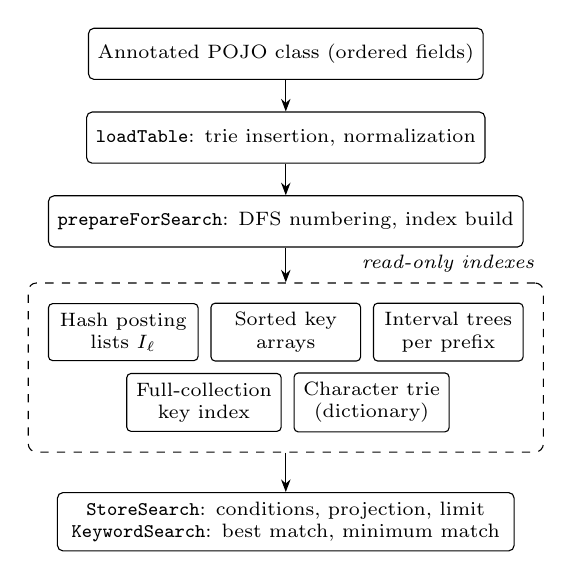
\begin{tikzpicture}[
  box/.style={draw, rounded corners=2pt, align=center, font=\scriptsize, minimum width=40mm, minimum height=6.5mm, fill=white},
  idx/.style={draw, rounded corners=1.5pt, align=center, font=\scriptsize, minimum width=19mm, minimum height=7mm, fill=white},
  arr/.style={-{Stealth[length=1.6mm]}, thin},
  node distance=4mm]
\node[box] (pojo) {Annotated POJO class (ordered fields)};
\node[box, below=of pojo] (load) {\texttt{loadTable}: trie insertion, normalization};
\node[box, below=of load] (prep) {\texttt{prepareForSearch}: DFS numbering, index build};
\node[idx, below=7mm of prep] (ord) {Sorted key\\arrays};
\node[idx, left=1.5mm of ord] (hash) {Hash posting\\lists $I_\ell$};
\node[idx, right=1.5mm of ord] (itv) {Interval trees\\per prefix};
\node[idx, below=1.5mm of hash, xshift=10.25mm] (full) {Full-collection\\key index};
\node[idx, right=1.5mm of full] (spell) {Character trie\\(dictionary)};
\node[draw, dashed, rounded corners=3pt, inner sep=2.5mm, fit=(hash)(ord)(itv)(full)(spell), label={[font=\scriptsize\itshape, anchor=south east]north east:read-only indexes}] (group) {};
\node[box, below=5mm of group, minimum width=58mm] (search) {\texttt{StoreSearch}: conditions, projection, limit\\\texttt{KeywordSearch}: best match, minimum match};
\draw[arr] (pojo) -- (load);
\draw[arr] (load) -- (prep);
\draw[arr] (prep) -- (group.north);
\draw[arr] (group.south) -- (search);
\end{tikzpicture}
\caption{Kiara components. All index structures are built once, after loading, and are read-only during search.}
\label{fig:architecture}
\end{figure}

\subsection{Schema Declaration and Value Normalization}
Table~\ref{tab:annotations} lists the seventeen indexing annotations. (The library spells several of them \emph{Seperated}.) Unannotated fields of string, character, Boolean, enumeration, and primitive or boxed numeric types are indexed as scalars. Normalization at load time and at query time maps every value to a key in one of two key spaces:
\begin{itemize}
\item \emph{String keys}: values are trimmed, lower-cased under \texttt{@CaseInsensitive}, stemmed under \texttt{@StemmedIndex}, and empty or null values map to a dedicated missing-value sentinel. Enumerations and Booleans use their textual form.
\item \emph{Numeric keys}: numeric scalars and numeric list elements map to 64-bit integers. Dates map to epoch days and date-times to UTC epoch seconds, using the format given in the annotation. Missing values map to a long sentinel.
\end{itemize}
The numeric mapping truncates fractional values through \texttt{Double.longValue()}, so 19.00, 19.50, and 19.99 share one key. Our oracle exposes the resulting differences in Section~\ref{sec:correctness}, and Section~\ref{sec:future} discusses an exact encoding. Node values retain the original number for result reconstruction.

\begin{table}[t]
\centering
\caption{Indexing Annotations in Kiara 2.0.16}
\label{tab:annotations}
\setlength{\tabcolsep}{3pt}
\renewcommand{\arraystretch}{1.08}
\begin{tabular}{@{}P{33mm}P{50mm}@{}}
\toprule
Annotation & Effect on indexing \\
\midrule
(none) & Scalar key, hash posting lists, sorted key array \\
\texttt{CaseInsensitive} & Lower-case at load and query time \\
\texttt{IgnoreIndex} & Stored and returned, but not searchable \\
\texttt{DateFormat}, \texttt{DateTimeFormat} & Epoch-day / UTC epoch-second numeric keys \\
\texttt{CS\{Strings, Numbers, Dates, DateTimes\}} & One key per element, plus a full-collection key \\
\texttt{NumericRange}, \texttt{DateRange}, \texttt{DateTimeRange} & Stored interval, optionally with a string prefix; prefix-partitioned interval tree \\
\texttt{CS\{NumericRanges, DateRanges, DateTimeRanges\}} & One stored interval per element \\
\texttt{StemmedIndex} & Snowball English stem at load and query time \\
\texttt{OneEditAway} & Keys added to the shared character trie used for correction and prediction \\
\texttt{Predictable} & Same effect as \texttt{OneEditAway} \\
\bottomrule
\multicolumn{2}{@{}p{0.95\columnwidth}@{}}{\footnotesize CS abbreviates the \texttt{CommaSeperated} prefix, so \texttt{CS\{Strings\}} denotes \texttt{CommaSeperatedStrings}.}
\end{tabular}
\end{table}

\subsection{Multi-Valued Attributes}
A collection-valued attribute, such as tags, sizes, observed markets, or a list of dates, occupies a single trie level. Its node value is the normalized collection. During the depth-first traversal, the node is appended to the posting list of \emph{every distinct element} and, separately, to a \emph{full-collection} index keyed by the whole collection. A node can therefore appear in several posting lists of the same level. Lemma~\ref{lem:levelorder} still guarantees that each list is sorted, because each list holds distinct same-level nodes appended in post-visit order. This extension keeps one logical index per attribute while supporting membership predicates without unnesting records into child rows, as the normalized relational designs evaluated in Section~\ref{sec:methodology} require.

\subsection{Ordered Keys for Comparisons}
Each level also keeps an array of its distinct keys, which is sorted once during preparation. \op{LESS\_THAN} and \op{LESS\_THAN\_EQUAL} scan the array forward until the bound fails. \op{GREATER\_THAN} and \op{GREATER\_THAN\_EQUAL} scan backward. \op{BETWEEN} binary-searches the lower bound and scans forward. Each qualifying key contributes its posting list to the candidate set. The work of a comparison is therefore proportional to the number of qualifying \emph{distinct keys}, not to the number of qualifying records. That cost is small for low-cardinality attributes and large for high-cardinality ones such as timestamps. A deprecated AVL-tree alternative (\texttt{SBTree}) remains in the code base but is unused.

\subsection{Stored Intervals}
Interval-valued attributes store ranges such as a capacity band \texttt{100-250}, a season \texttt{2026-06-01..2026-08-31}, or a prefixed range \texttt{AA10-1004}. With \texttt{numericStartPos}$=2$, the last example is partitioned under prefix \texttt{AA} with numeric interval $[10,1004]$. Each level keeps one interval tree per prefix. Preparation sorts the distinct intervals by lower endpoint and builds a perfectly balanced binary search tree by recursive midpoint selection. It then augments every node with the maximum upper endpoint in its subtrees, which is the classical interval-tree augmentation~\cite{cormen2009introduction}. A point query on a stored interval, the stabbing query used by \op{CONTAINS\_EITHER} and \op{CONTAINS\_ALL}, skips the left subtree when the point lies below a node's lower endpoint. It prunes both subtrees when the point exceeds the maximum upper endpoint recorded for them. Pruning is effective in practice, but this traversal's worst case remains $O(n)$ for $n$ distinct intervals. Each stabbed interval maps through its canonical string to a posting list of trie nodes. For lists of intervals, every element is indexed separately, so the endpoints of one interval are never paired with those of another, which preserves interval correlation.

Kiara~2.0.15 compared interval lower bounds with reference equality on boxed \texttt{Long} values. Java caches boxed values only in a small range, so the comparator was inconsistent for repeated large lower bounds such as epoch seconds. Sorting larger schedules then failed with a ``comparison method violates its general contract'' error. Version~2.0.16 compares the primitive values. Our benchmark exposed this defect, and its fix is a precondition for the schedule results in Section~\ref{sec:results}.

\subsection{Operators}
Table~\ref{tab:operators} lists the eleven operators and how each produces its candidate set at one level. The rightmost column is the candidate \emph{fan-out} $q$, the number of sorted posting lists in the candidate collection. Section~\ref{sec:cost} shows that $q$ governs much of the cost of a query. Negations are evaluated over the key space of the level rather than as a set difference over records. \op{NOT\_EQUAL} enumerates every key except the excluded ones. \op{NOT\_CONTAINS}, which applies only to collections, first marks every full-collection key that contains an excluded element and then enumerates the remaining full-collection keys. Comparisons and \op{BETWEEN} on interval attributes are rejected. A predicate on a missing value is expressed with the null literal, which normalization maps to the sentinel key.

\begin{table*}[t]
\centering
\caption{Operators, Candidate Generation, and Candidate Fan-Out at One Level}
\label{tab:operators}
\setlength{\tabcolsep}{4pt}
\renewcommand{\arraystretch}{1.08}
\begin{tabular}{@{}P{46mm}P{88mm}P{36mm}@{}}
\toprule
Operator & Candidate generation & Fan-out $q$ (lists) \\
\midrule
\op{EQUAL} & Hash lookup per requested value (interval attributes: canonical interval string) & $\le$ requested values \\
\op{CONTAINS\_EITHER} & As \op{EQUAL}; on interval attributes, one stabbing query per requested point & requested values; stabbed intervals \\
\op{CONTAINS\_EITHER\_}\allowbreak\op{INCLUDING\_NULL} & Rewritten to \op{CONTAINS\_EITHER} over the requested values plus the missing-value key & requested values $+1$ \\
\op{CONTAINS\_ALL} & Intersection of per-element lists; on interval attributes, stabbed lists are merged per point and then intersected & $1$ \\
\op{NOT\_EQUAL} & Enumerate all keys of the level except the requested values & distinct keys $-$ requested \\
\op{NOT\_CONTAINS} (collections) & Mark full-collection keys containing a requested element; enumerate the rest & distinct collections $-$ marked \\
\op{LESS\_THAN}, \op{LESS\_THAN\_EQUAL} & Forward scan of the sorted key array & qualifying distinct keys \\
\op{GREATER\_THAN}, \op{GREATER\_THAN\_EQUAL} & Backward scan of the sorted key array & qualifying distinct keys \\
\op{BETWEEN} & Binary search to the lower bound, then forward scan (inclusive) & qualifying distinct keys \\
\bottomrule
\end{tabular}
\end{table*}

\subsection{Query Evaluation over Disjunctive Posting-List Collections}
\label{sec:reduction}
Kiara represents every intermediate result as a \emph{collection} $\mathcal{C}=\{L_1,\dots,L_q\}$ of sorted node lists whose union is the candidate set. Disjunctive predicates such as multi-value \op{EQUAL}, comparisons, and negations therefore require no merge step: each qualifying key contributes its existing posting list by reference. Algorithm~\ref{alg:reduction} shows the evaluation, which proceeds in three steps.
\begin{enumerate}
\item Conditions are sorted by level, so the trie is visited from the root downward. In version~2.0.16 the order is structural; it does not depend on selectivity.
\item Several conditions on the same level are combined by hash-based intersection of their candidate sets.
\item Consecutive constrained levels are combined by a structural join that adapts its direction to the candidate sizes. If the deeper candidate set is smaller, \textsc{ProbeUp} keeps each deeper node for which some current list contains an ancestor, found by binary search on interval containment (Lemma~\ref{lem:ancestry}). Otherwise, \textsc{ExpandDown} visits each current node and, in each deeper list, binary-searches the contiguous run of its descendants (Lemma~\ref{lem:levelorder}), merging the runs found in different lists.
\end{enumerate}
A hash set suppresses duplicate visits to nodes of the shallower side, because a node can occur in several lists. A descendant that occurs in several deeper lists can be emitted more than once, and such duplicates are removed during materialization. An empty candidate set terminates evaluation early. The 2020 design used only the \textsc{ProbeUp} direction over single lists. The collection representation and \textsc{ExpandDown} were added to support the operators of Table~\ref{tab:operators}.

\begin{algorithm}[t]
\caption{Adaptive Level-Wise Reduction}
\label{alg:reduction}
\begin{algorithmic}[1]
\Require Conditions grouped by level; level indexes
\Ensure Collection $\mathcal{R}$ of sorted node lists at the deepest constrained level
\State $\mathcal{R}\gets\bot$
\For{each constrained level $\ell$, in increasing order}
  \State $\mathcal{C}\gets\textsc{Candidates}(q_{\ell,1})$ \Comment{Table~\ref{tab:operators}}
  \For{each further condition $q_{\ell,j}$ on level $\ell$}
    \State $\mathcal{C}\gets\textsc{HashIntersect}(\mathcal{C},\textsc{Candidates}(q_{\ell,j}))$
  \EndFor
  \If{$\mathcal{C}=\emptyset$}
    \State \Return $\emptyset$
  \EndIf
  \If{$\mathcal{R}=\bot$}
    \State $\mathcal{R}\gets\mathcal{C}$
  \ElsIf{$\|\mathcal{C}\|<\|\mathcal{R}\|$} \Comment{$\|\cdot\|$: total nodes}
    \State $\mathcal{R}\gets\textsc{ProbeUp}(\mathcal{R},\mathcal{C})$
  \Else
    \State $\mathcal{R}\gets\textsc{ExpandDown}(\mathcal{R},\mathcal{C})$
  \EndIf
\EndFor
\State \Return $\mathcal{R}$
\Statex
\Function{ProbeUp}{$\mathcal{R},\mathcal{C}$}
  \For{each distinct node $v$ in the lists of $\mathcal{C}$}
    \If{a binary search finds an ancestor of $v$ in some $L\in\mathcal{R}$}
      \State emit $v$
    \EndIf
  \EndFor
\EndFunction
\Function{ExpandDown}{$\mathcal{R},\mathcal{C}$}
  \For{each distinct node $u$ in the lists of $\mathcal{R}$}
    \State $\mathit{runs}\gets$ descendant run of $u$ in each $L\in\mathcal{C}$
    \State emit the $\pre$-ordered merge of $\mathit{runs}$
  \EndFor
\EndFunction
\end{algorithmic}
\end{algorithm}

\subsection{Result Materialization}
For each node $v\in\mathcal{R}$, Kiara walks parent pointers upward to the shallowest projected attribute. It then enumerates every root-to-leaf continuation below $v$ by recursive descent, emitting one result per leaf path. Results are either reconstructed POJOs, populated through reflection, or maps restricted to the requested projection. An optional limit stops emission once reached. The limit is applied during materialization, after the candidate collection has been fully computed. Section~\ref{sec:cost} shows why this matters for broad queries.

\subsection{Text Retrieval Layer}
\label{sec:text}
Interactive search must tolerate how people type. Kiara builds its text features from the same level indexes rather than from a separate document index.

\paragraph*{Tokenization and stemming}
Keyword input is split on single space characters after punctuation is replaced by spaces and brackets are removed, and duplicate terms are discarded. Despite its name, the routine \texttt{removeStopWords} performs no stop-word filtering. Attributes annotated with \texttt{@StemmedIndex} store Snowball English stems~\cite{porter2001snowball} of their keys, and query terms are stemmed per attribute before lookup. A query term may therefore match the stemmed form in one attribute and the literal form in another.

\paragraph*{One-edit correction}
Keys of attributes annotated with \texttt{@OneEditAway} or \texttt{@Predictable} are inserted into a character trie with a terminal marker. Correction applies only to terms longer than three characters and walks the trie along the input. At the first mismatch, it tries a deletion of the input character, then an insertion, by matching the input character against grandchildren of the current node, and then a substitution, by matching the next input character against grandchildren. At the end of the input it may also complete a word one character short. It fails if more than one edit is required. The walk is greedy and follows a single path: it returns at most one correction, at Levenshtein distance one~\cite{levenshtein1966binary}, in $O(|w|\,\sigma)$ time for alphabet fan-out $\sigma$. It does not guarantee that a correction is found whenever one exists, and it does not rank alternatives. Levenshtein automata~\cite{schulz2002fast} or BK-trees~\cite{burkhard1973approaches} trade more index work for completeness. Kiara chooses predictability and constant memory per dictionary character.

\paragraph*{Prefix prediction}
Type-ahead walks the character trie to the node for the typed prefix and then traverses its subtree breadth-first. It emits completed words in non-decreasing length up to a requested count. The cost is $O(|p|)$ plus the number of trie nodes visited. Predictions are dictionary words, not records, which keeps suggestion separate from filtering. Predictions are not ranked by popularity.

\paragraph*{Coverage-maximizing keyword search}
\texttt{KeywordSearch.getBestMatch} accepts free text and optional hard conditions, for example ``in stock'' or ``region = EMEA''. It must decide which attribute each keyword refers to. Algorithm~\ref{alg:keyword} gives a simplified form of the procedure. Each keyword is first bound to the set $F(w)$ of levels whose index contains its form after that level's normalization. A keyword with no binding is replaced by its one-edit correction when one exists. Each assignment of keywords to levels then defines a structured conjunction, with one \op{CONTAINS\_ALL} condition per level plus the hard conditions, which is evaluated by Algorithm~\ref{alg:reduction}. Conjunctions are tried in order of decreasing keyword coverage, and the first non-empty result is returned together with the keywords it satisfied. This semantics is \emph{coverage-first}: a result that matches more of the user's words always wins, and dropped words are reported rather than silently ignored. Within one coverage level, the result depends on enumeration order, which follows hash-based collections and is therefore implementation-dependent; Kiara does not compute TF-IDF or BM25 scores~\cite{robertson2009bm25}. The number of conjunctions is bounded by $\prod_{w}(|F(w)|+1)$, and a constructor parameter caps the number of keywords considered.

Version~2.0.16 has one limitation that matters for correctness. Kiara records \emph{one} representative form $\tilde w$ per keyword: the normalized form from the last level that matched. It then queries every bound level with $\tilde w$. When a term matches a raw attribute literally and a stemmed attribute through its stem, conditions on the raw attribute receive the stem, which can miss records (Section~\ref{sec:correctness}). Retaining a normalized key per bound level removes this defect.

\texttt{getMinimumMatch} post-filters best-match results with a cardinality test. A record passes when the number of distinct populated non-numeric attribute values equals the number of matched keywords. The test is intended for hierarchical configuration lookup, where the most specific rule should match a request and broader rules should not. However, it compares counts rather than value sets and does not tokenize collection values, so it only approximates that semantics.

\begin{algorithm}[t]
\caption{Coverage-Maximizing Keyword Search (Simplified)}
\label{alg:keyword}
\begin{algorithmic}[1]
\Require Text $s$, hard conditions $H$, limit $\lambda$
\Ensure Matched keywords and records
\State $W\gets\textsc{Tokenize}(s)$
\For{each $w\in W$}
  \State $F(w)\gets\{\ell : \nu_\ell(w)\in\mathrm{keys}(I_\ell)\}$ \Comment{$\nu_\ell$: case folding, stemming}
  \State $\tilde w\gets\nu_{\max F(w)}(w)$ \Comment{one form per keyword in 2.0.16}
  \If{$F(w)=\emptyset$ and $w'\gets\textsc{OneEdit}(w)$ exists, $w'\notin W$}
    \State replace $w$ by $w'$; recompute $F(w')$ and $\tilde w'$
  \EndIf
\EndFor
\State $W^\ast\gets\{w : F(w)\neq\emptyset\}$
\For{$c\gets|W^\ast|$ \textbf{down to} $1$}
  \For{each assignment $\sigma$ of $c$ keywords to levels with $\sigma(w)\in F(w)$}
    \State $Q\gets H\cup\{\op{CONTAINS\_ALL}(\ell,\{\tilde w:\sigma(w)=\ell\})\}_\ell$
    \State $R\gets\textsc{Search}(Q,\lambda)$ \Comment{Algorithm~\ref{alg:reduction}}
    \If{$R\neq\emptyset$}
      \State \Return $(\mathrm{dom}(\sigma), R)$
    \EndIf
  \EndFor
\EndFor
\State \Return $(\emptyset,\emptyset)$
\end{algorithmic}
\end{algorithm}

\subsection{Evolution of the Implementation}
Table~\ref{tab:releases} summarizes the releases. Version~1.0.0, contemporaneous with~\cite{kapoor2020efficient}, already contained the typed, collection, and interval machinery, but that article described only equality search. The text layer and the remaining interface features followed in 2020--2021. Maintenance releases in 2026 modernized dependencies and fixed the interval comparator. The repository contains 461 JUnit test methods in 45 test files. A TypeScript port~\cite{kiarats2026software}, aligned with version~2.0.16 through live Java-versus-TypeScript differential tests, shows that the model is not tied to the JVM.

\begin{table}[t]
\centering
\caption{Release History of the Java Library}
\label{tab:releases}
\setlength{\tabcolsep}{2.5pt}
\renewcommand{\arraystretch}{1.05}
\begin{tabular}{@{}llP{56mm}@{}}
\toprule
Version & Date & Principal change \\
\midrule
1.0.0 & 2020-05 & Typed, collection, interval attributes; 11 operators \\
1.2.0 & 2020-11 & Keyword search, Snowball stemming, one-edit trie \\
2.0.0 & 2021-01 & Type-checked loading; keyword-search API \\
2.0.4 & 2021-01 & Thread-safe keyword search \\
2.0.5--6 & 2021-02 & Result limits for structured and keyword search \\
2.0.8 & 2021-02 & Case-insensitive attributes \\
2.0.9 & 2021-02 & \texttt{@Predictable} type-ahead \\
2.0.10 & 2021-03 & Minimum-match keyword search \\
2.0.12 & 2021-05 & Enumeration attributes \\
2.0.15 & 2026-10 & Dependency and build modernization \\
2.0.16 & 2026-10 & Interval comparator contract fix \\
\bottomrule
\end{tabular}
\end{table}

\section{Cost Model}
\label{sec:cost}

The worst-case bound of~\cite{kapoor2020efficient}, $O(KMN\log N)$, is too coarse to explain measured behavior. Here we model costs in terms of quantities that vary across queries. For a store, let $N$ be the number of records and $m$ the number of attributes. For a candidate collection $\mathcal{C}$, let $\|\mathcal{C}\|$ be its total number of nodes, $q_{\mathcal{C}}$ the number of lists (its fan-out), and $\Lambda_{\mathcal{C}}$ its longest list.

\subsection{Build Cost}
Trie insertion locates the child of the current node that carries the next value. In version~2.0.16 this is a \emph{linear} scan over the children of the current node that compares normalized string keys. Inserting a record costs $\sum_{\ell}\deg(v_{\ell-1})$, where each degree is the fan-out at insertion time. If a near-unique attribute, such as a record identifier, occupies level~1, the root fan-out grows to $N$ and loading costs $\Theta(N^2)$ comparisons. Hashing children by key reduces insertion to $O(Nm)$ expected time. The depth-first numbering visits each node once and appends it to one posting list per distinct key, which is linear in the index size. Sorting key arrays and building interval trees adds $O(d\log d)$ per level for $d$ distinct keys or intervals. Unique-first placement also disables prefix sharing below level~1, so the trie holds roughly $Nm$ nodes.

The library documentation recommends placing high-cardinality attributes deep in the schema, where they cost little. Our benchmark schema instead places the identifier first, because one annotated record class is shared by all engines (Section~\ref{sec:methodology}). Under the quadratic model, a 10$\times$ larger fixture should build about 100$\times$ more slowly. We observed 113--159$\times$ for Kiara, from 1.15--1.50\,s at 10{,}000 records to 158--183\,s at 100{,}000 across two suites, against about 4$\times$ for Lucene (Section~\ref{sec:lucene}). The additional factor is consistent with growing garbage-collection and cache pressure. Kiara's TypeScript port keys children by hash map. In an equivalent-workload Java-versus-TypeScript benchmark that ships with the port~\cite{kiarats2026software}, it prepared 100{,}000 records in 0.76\,s, compared with 470\,s for the Java library. That benchmark uses a different schema and a different runtime, so the comparison is indicative only. It is nevertheless consistent with the view that the build cost is a property of the Java implementation rather than of the model.

\subsection{Query Cost}
\paragraph*{Candidate generation} Equality and \op{CONTAINS\_EITHER} cost one hash lookup per requested value. Comparisons and \op{BETWEEN} cost $O(\log d + q)$ and reference $q$ existing lists without copying them. \op{NOT\_EQUAL} costs $O(d_\ell)$. \op{NOT\_CONTAINS} costs $O(D_\ell+\sum_x|P_\ell(x)|)$ for $D_\ell$ distinct collection values, because it first visits the postings of each excluded element $x$. \op{CONTAINS\_ALL} repeatedly intersects sorted element lists with a two-pointer merge. A stabbing query costs $O(n)$ in the worst case, although pruning usually visits far fewer nodes, plus the merge of the stabbed lists when they must be combined.

\paragraph*{Reduction} From Algorithm~\ref{alg:reduction},
\begin{align}
T_{\textsc{ProbeUp}}    &= O\!\left(\|\mathcal{C}\|\; q_{\mathcal{R}} \log \Lambda_{\mathcal{R}}\right), \label{eq:probeup}\\
T_{\textsc{ExpandDown}} &= O\!\left(\|\mathcal{R}\|\; q_{\mathcal{C}} \log \Lambda_{\mathcal{C}} + q_{\mathcal{C}}\,\mathit{out}\right), \label{eq:expanddown}
\end{align}
where $\mathit{out}$ is the number of descendants emitted. The second term bounds the cost of merging each new run into the accumulated runs, one list at a time. The algorithm takes the cheaper side with respect to $\|\cdot\|$. When both sides have fan-out one, as with single-value equality or \op{CONTAINS\_ALL}, Eqs.~\eqref{eq:probeup}--\eqref{eq:expanddown} reduce to the classical smaller-probes-larger bound $O(\min(|A|,|B|)\log\max(|A|,|B|))$~\cite{baezayates2004fast}, applied to trie nodes rather than to records. When the side being probed has a large fan-out, the cost grows \emph{multiplicatively} in that fan-out. The direction is chosen by node counts alone, so a high-fan-out probed side is not avoided. Same-level intersection is linear in the sizes of both candidate sets regardless of how small their intersection is.

\paragraph*{Materialization} Each result costs $O(m)$ pointer traversals plus object construction. A limit bounds only this phase.

\subsection{Predicted Strengths and Weaknesses}
\label{sec:predictions}
The model yields six testable predictions, which Section~\ref{sec:results} examines.
\begin{enumerate}
\item[P1] \emph{Collection membership is cheap.} \op{CONTAINS\_ALL} and few-value \op{CONTAINS\_EITHER} have small fan-out and short lists. The normalized relational designs we evaluate instead join child rows and deduplicate or group them.
\item[P2] \emph{High-fan-out predicates are expensive when the other side is large.} Negations over many distinct collections, and stabbing queries that hit many distinct stored intervals, produce thousands of lists. Pairing them with a broad predicate on another level triggers Eq.~\eqref{eq:expanddown} with a large $q_{\mathcal{C}}$.
\item[P3] \emph{Same-attribute windows are expensive.} Writing a window as two comparisons on one high-cardinality attribute generates two broad candidate sets and intersects them, even when the window contains few records. A single \op{BETWEEN} generates only the qualifying keys.
\item[P4] \emph{Conjunctions of broad scalar predicates scale poorly.} Ordering by level rather than by selectivity, together with the absence of compound access paths, makes the cost track the sum of candidate sizes. A compound B-tree seek tracks only the output size.
\item[P5] \emph{Limits do not reduce candidate work.} A limit cannot make the candidate phase cheaper than the full query.
\item[P6] \emph{Build time is quadratic under unique-first schemas,} as derived above.
\end{enumerate}

\section{Experimental Methodology}
\label{sec:methodology}

The evaluation asks two questions. Where does the attribute-trie design reduce query latency relative to mature alternatives? Where, and why, does it not? Our design goals were \emph{semantic equivalence before speed}, \emph{fair physical design for every opponent}, and \emph{full disclosure of exclusions}. All harnesses, raw per-trial samples, plans, index inventories, and reports are publicly available (see the data availability statement).

\subsection{Systems and Configurations}
Table~\ref{tab:suites} lists the seven suites. Kiara~2.0.16 was used unmodified throughout. Opponents were Apache Lucene~10.5.2; SQLite~3.53.4 through the Xerial JDBC driver~3.53.4.0~\cite{gaffney2022sqlite}; and VoltDB Community Edition~10.1.1, the last AGPL release, from 2020~\cite{stonebraker2013voltdb}. The VoltDB results do not describe current commercial VoltDB.

\emph{Tuned} configurations received workload-specific physical design. Tuned SQLite used 38 indexes: 17 covering scalar indexes, 4 interval-bound indexes, 5 list owner, value, and interval indexes, 11 compound indexes for the tested conjunctions, and the primary key. It also ran a full \texttt{ANALYZE} and froze, per query, the fastest of 197 validated SQL alternatives (indexed joins, \texttt{IN}, \texttt{EXISTS}/\texttt{NOT EXISTS}, \texttt{EXCEPT}, \texttt{INTERSECT}). Tuned VoltDB used precompiled read-only single-partition procedures with replicated data, 37 verified indexes, and the fastest of 184 candidates, one of which timed out and was excluded. Frozen plans had to match final plans.

\emph{Generic} configurations retained per-attribute indexes but no workload-specific compound indexes or SQL search: 26 indexes and no \texttt{ANALYZE} for SQLite, and one predetermined SQL statement per query for VoltDB. ``Generic'' therefore does not mean unindexed. Kiara's schema and query formulations were held fixed in every suite. Kiara received no query-specific tuning, so the tuned suites deliberately favor the opponents.

\begin{table*}[t]
\centering
\caption{Benchmark Suites. Ratios in Section~\ref{sec:results} Are Opponent Latency Divided by Kiara Latency}
\label{tab:suites}
\setlength{\tabcolsep}{3.5pt}
\renewcommand{\arraystretch}{1.1}
\begin{tabular}{@{}lP{44mm}P{74mm}lP{22mm}@{}}
\toprule
Suite & Opponent configuration & Timed region (both engines unless noted) & Trials & Datasets \\
\midrule
S1 & Lucene, \texttt{ByteBuffersDirectory}, query cache off, numeric points and \texttt{LongRange} & In-process query construction, execution, materialization, ID extraction & 3 forks & Base five \\
S2 & VoltDB, client--server, parameterized ad hoc SQL, generic indexes & Client-visible: transport, execution, fetch, decoding & 3 forks & Base five \\
S3 & VoltDB, tuned & Server-side SQL execution and \texttt{VoltTable} creation inside a procedure; Kiara: search and eager result maps & 5 & Base five \\
S4 & VoltDB, generic & As S3 & 5 & Base five, wide \\
S5 & SQLite, tuned, private \texttt{:memory:} database & Prepared execution, all cursor steps, JDBC/JNI conversion, eager result maps & 5 & Base five \\
S6 & SQLite, generic; 60\,s per-call deadline for both engines & As S5 & 5 & Base five \\
S7 & VoltDB tuned, SQLite tuned and generic, Lucene & Per-pair boundaries as above; Lucene constant-score retrieval, document order & 5 & Wide \\
\bottomrule
\end{tabular}
\end{table*}

\subsection{Datasets and Workloads}
Table~\ref{tab:datasets} summarizes the fixtures. The retail fixture is a projection of the UCI Online Retail dataset~\cite{chen2015online}, licensed CC BY 4.0. It contains 3,788 genuine stock codes with historical prices, units sold, and the list of countries in which each product sold, aggregated from 525,462 qualifying transactions among 541,909 source rows. Catalog and schedule fixtures are generated from fixed seeds with skewed, nullable, list-valued, and interval-valued attributes. The wide fixtures vary the number of \emph{distinct} filtered attributes from 2 to 16 at target selectivities of 0.1\%, 1\%, and 10\%, giving 39 queries per fixture. Non-selector predicates accept 95\% of rows, and 90\% for \op{CONTAINS\_ALL}, so that width adds real, mostly broad predicates. Scalar-only controls stop at eight attributes, the number of applicable scalar fields. All engines receive identical input objects from one annotated record class with 27 attributes. Attributes irrelevant to a family are null.

The base workload comprises 60 scenarios in 12 categories: equality, numeric comparisons, lists, missing values, typed scalars, dates and times, date and time lists, stored ranges, combined conjunctions, result shaping, text, and dictionary operations. Together they exercise all eleven operators and all seventeen annotations.

\begin{table}[t]
\centering
\caption{Datasets}
\label{tab:datasets}
\setlength{\tabcolsep}{3pt}
\begin{tabular}{@{}lrP{50mm}@{}}
\toprule
Fixture & Records & Characteristics \\
\midrule
retail & 3,788 & Real UCI projection; market lists, fractional prices, titles \\
catalog & 10k, 100k & Status, region, tier, sale, supplier, prices, tags, sizes, titles \\
schedule & 10k, 100k & Dates, timestamps, date/time lists, numeric, prefixed, date, and time ranges \\
wide & 10k, 100k & 2--16 distinct attributes; 0.1/1/10\% selectivity \\
\bottomrule
\end{tabular}
\end{table}

\subsection{Correctness Oracle and Eligibility}
\label{sec:oracle}
Before warm-up, every timed scenario was checked against an engine-independent scan oracle for matched IDs, counts, and result shape. In S7, results were checked again after timing. Unexpected mismatches aborted the run instead of producing samples. Recognized semantic differences were labeled, retained, and excluded from speed aggregates:
\begin{itemize}
\item \textsc{Known\_Decimal\_Truncation}: Kiara's integer keys for fractional numbers (Section~\ref{sec:system}), accepted only when the exact truncation model predicted the mismatch.
\item \textsc{Text\_Result\_Difference}: keyword outputs that differ from the intended-token oracle.
\item \textsc{Unsupported}: the SQL adapters have no equivalent text, prediction, or correction operation. These modes were timed for neither engine, which is not a statement about the SQL engines' full-text features.
\item Limited queries can return different valid subsets; they were validated but excluded from ratios.
\item \textsc{Query\_Timeout} and \textsc{Build\_Failed}: recorded as outcomes, never as fabricated latencies.
\end{itemize}
Only queries that returned oracle-equivalent results in every trial of both engines entered a ratio.

\subsection{Protocol and Statistics}
Each trial ran in a fresh JVM. In S3--S7, each trial also ran in a fresh Linux container with a four-CPU quota, an 8\,GiB memory limit, and a 1--4\,GiB Java heap. VoltDB was restarted before every trial, data were rebuilt outside the timed region, engine order alternated, and scenario order was shuffled reproducibly. Warm-up comprised at least ten calls and 1\,s, followed by 15--101 measured calls within a 3\,s acquisition budget. S1 and S2 used three forks, at least three warm-up queries, and 5--61 samples within a 1\,s budget. Kiara and Lucene workers used JDK~21. The legacy VoltDB server required JDK~11. All suites ran on one shared, virtualized AMD EPYC 7763 host.

For each query we took the median across trials of the per-trial nearest-rank p50. The per-query ratio is opponent latency divided by Kiara latency, so values above one favor Kiara. A dataset-level ratio is the unweighted geometric mean of eligible per-query ratios~\cite{fleming1986how}. Its exploratory 95\% interval is a percentile bootstrap~\cite{efron1993introduction} over 5,000 whole-trial resamples with a fixed seed, which preserves within-trial correlation between queries. With five trials these intervals describe trial variability for a fixed workload. They do not establish generality. The seven suites recorded 1,042,491 raw latency samples, including tuning-candidate samples.

\section{Results}
\label{sec:results}

\subsection{Kiara Versus Lucene (S1)}
\label{sec:lucene}
Table~\ref{tab:lucene} reports the in-process comparison. Kiara had lower aggregate latency on equivalent structured queries for all five datasets, from 3.46$\times$ on the 100,000-event schedule to 16.07$\times$ on the 10,000-product catalog. For keyword scenarios that returned equivalent results in every fork, the corresponding ratios were 2.15--6.05$\times$. The aggregates weight each query equally, and Kiara did not win every individual query. The suite recorded 738 scenario--fork measurements and 37,110 samples, and all 30 worker builds succeeded.

The cost is on the build side. At 10,000 records, build times were similar. At 100,000 records, Lucene built its index 38$\times$ (catalog) and 26$\times$ (schedule) faster. Lucene also retained 11--20$\times$ less additional heap, measured as post-build heap growth after requested garbage collection. As Section~\ref{sec:cost} predicts, Kiara's build cost under the shared unique-first schema is quadratic. Unique-first placement also removes prefix sharing, so the memory figures represent an unfavorable layout for Kiara rather than its best case.

\begin{table}[t]
\centering
\caption{Kiara Versus Lucene (S1): Aggregate Lucene/Kiara Latency Ratios, Build Time, and Additional Retained Heap}
\label{tab:lucene}
\setlength{\tabcolsep}{2pt}
\begin{tabular}{@{}lrrrcc@{}}
\toprule
Dataset & Eq. & Struct. & Kw. & Build s (K/L) & Heap MiB (K/L) \\
\midrule
retail 3,788 & 5 & 7.98 & 2.15 & 0.49/0.67 & 14.1/0.7 \\
catalog 10k & 22 & 16.07 & 6.05 & 1.15/1.12 & 33.5/2.1 \\
catalog 100k & 22 & 9.43 & 4.63 & 183.0/4.76 & 327.4/20.0 \\
schedule 10k & 22 & 5.42 & -- & 1.30/1.46 & 33.4/2.9 \\
schedule 100k & 22 & 3.46 & -- & 157.6/6.00 & 294.4/27.0 \\
\bottomrule
\multicolumn{6}{@{}p{0.95\columnwidth}@{}}{\footnotesize Eq.: equivalent structured scenarios; Kw.: equivalent-keyword ratio. Schedule fixtures contain no keyword workloads.}
\end{tabular}
\end{table}

\subsection{Kiara Versus SQL Engines (S2--S6)}
Table~\ref{tab:sql} summarizes the five SQL configurations. Three patterns stand out.

\emph{First, the timing boundary matters as much as the engine.} In the client--server configuration (S2), Kiara had 2.86--67.64$\times$ lower aggregate latency. Removing transport and client decoding (S3) moved the 100,000-record aggregates in VoltDB's favor (0.80 and 0.92). A comparison between an embedded library and a server therefore depends on whether the application actually pays network costs.

\emph{Second, generic physical design favors Kiara.} Against generic-index configurations (S4, S6), Kiara had lower aggregate latency in eleven of twelve dataset entries. The exception was the 100,000-event schedule against SQLite (0.94). On generic SQLite, Kiara also completed two queries that SQLite could not finish within the 60\,s deadline in any trial, \texttt{tags-exclude} on the large catalog and \texttt{range-list-point} on the large schedule. These outcomes are counted separately and are not converted into latencies.

\emph{Third, workload-specific tuning reverses the large-dataset results.} Tuned SQLite reached 0.30--0.69 on three of five datasets and tuned VoltDB 0.80--0.99 on three. Kiara nevertheless retained more lower per-query medians than either tuned engine on most fixtures. Against tuned VoltDB, Kiara had lower medians on 46 of 89 dataset--query pairs and VoltDB on 43. Against tuned SQLite the count was 54 of 89 for Kiara and 35 for SQLite. The aggregates are dominated by the \emph{magnitude} of a few losses, which Section~\ref{sec:anatomy} examines.

\begin{table*}[t]
\centering
\caption{Aggregate Opponent/Kiara Latency Ratios Against SQL Engines (Geometric Means; Exploratory 95\% Bootstrap Intervals in Parentheses). Values Above 1 Favor Kiara}
\label{tab:sql}
\setlength{\tabcolsep}{4pt}
\renewcommand{\arraystretch}{1.1}
\begin{tabular}{@{}lrrrrrr@{}}
\toprule
Dataset & Queries & S5 SQLite tuned & S6 SQLite generic & S3 VoltDB tuned & S4 VoltDB generic & S2 VoltDB client--server \\
\midrule
retail 3,788 & 5 & 5.30 (4.83--6.47) & 11.57 (8.52--12.65) & 10.95 (8.98--12.46) & 28.60 (21.92--31.88) & 67.64 \\
catalog 10k & 21 & 1.68 (1.43--1.74) & 3.33 (3.15--3.52) & 0.99 (0.89--1.13) & 1.52 (1.38--1.62) & 8.16 \\
catalog 100k & 21 & 0.61 (0.54--0.68) & 1.76 (1.59--1.83)$^{\ast}$ & 0.80 (0.71--0.86) & 1.14 (1.07--1.27) & 2.86 \\
schedule 10k & 21 & 0.69 (0.65--0.73) & 2.02 (1.94--2.09) & 1.32 (1.23--1.47) & 2.45 (2.30--2.60) & 10.88 \\
schedule 100k & 21 & 0.30 (0.29--0.31) & 0.94 (0.85--0.97)$^{\ast}$ & 0.92 (0.85--0.99) & 1.89 (1.75--2.00) & 4.66 \\
wide 10k & 39 & -- & -- & -- & 15.43 (15.06--16.79) & -- \\
wide 100k & 39 & -- & -- & -- & 10.99 (10.49--11.34) & -- \\
\bottomrule
\end{tabular}
\par\vspace{1mm}\parbox{0.97\textwidth}{\footnotesize $^{\ast}$20 fully measured queries; the remaining query was a deadline-completion win for Kiara. S2 used three forks and reported no intervals, and its equivalent-query sets were 5/22/22/22/22. S2 build times (Kiara/VoltDB) were 0.45/6.92\,s, 1.21/8.98\,s, 177.2/48.7\,s, 1.50/8.42\,s, and 169.6/46.5\,s in the order listed.}
\end{table*}

\subsection{Anatomy of the Extremes}
\label{sec:anatomy}
Table~\ref{tab:anatomy} lists representative 100,000-record queries against tuned VoltDB, together with the prediction from Section~\ref{sec:predictions} that accounts for each. The VoltDB plans used compound indexes, bounded index scans, and indexed set differences.

\emph{Collection membership (P1).} Queries over tags, sizes, date lists, and timestamp lists, and point-in-interval queries over stored durations, ran 16.8--70.5$\times$ faster in Kiara. On the retail fixture, ``markets contain both values'' ran 33.3$\times$ faster and ``markets exclude a value'' 25.2$\times$ faster. The relational formulations must join child rows and then group, deduplicate, or apply conditional aggregation. An index does not remove that work. Kiara intersects two short posting lists at one level.

\emph{High-fan-out predicates paired with broad ones (P2).} The worst result, ``active status and tags exclude clearance,'' took 14.2\,s in Kiara against 0.21\,s in VoltDB, and was consistent across trials (13.4--17.7\,s). \op{NOT\_CONTAINS} enumerates every distinct tag collection, which yields thousands of lists. The status predicate sits higher in the trie and matches most records, so \textsc{ExpandDown} performs one binary search per pair of status node and tag list, as Eq.~\eqref{eq:expanddown} predicts. The season query (8.8\,s against 45\,ms) has the same structure, because a stabbing query over many distinct season intervals meets a broad event-type predicate. On the small retail fixture the same operator was a strength, because neither side was large. Exclusion is therefore not intrinsically slow in Kiara. Its cost depends on the fan-out and on what it is paired with.

\emph{Same-attribute windows (P3).} The four-hour timestamp window returned 77 events. Kiara took 30.3\,ms, because two broad comparisons on a high-cardinality attribute were each materialized as candidate collections and then intersected. VoltDB took 40\,\textmu s with one bounded index scan. Kiara's \op{BETWEEN} operator generates only the qualifying keys. The benchmark fixed the two-predicate form in advance, so this ratio applies to that formulation.

\emph{Broad scalar conjunctions (P4).} ``Status and region and brand'' took 6.5\,ms in Kiara and 0.13\,ms in VoltDB, which sought a compound index on (brand, status, region, id). This is precisely the access path that Proposition~\ref{prop:indexcount} shows cannot exist for \emph{every} combination. For a fixed, known combination, however, it wins decisively.

\emph{Limits (P5).} ``First 20 active products'' took 39.8\,ms in Kiara against 27\,\textmu s in tuned SQLite (S5), which stops scanning after 20 rows. Limited queries were excluded from the ratios because no ordering contract defines a unique answer.

\begin{table}[t]
\centering
\caption{Representative 100k-Record Queries Against Tuned VoltDB (S3), Median p50 Execution Time}
\label{tab:anatomy}
\setlength{\tabcolsep}{1.8pt}
\begin{tabular}{@{}lrrrc@{}}
\toprule
Query & Kiara ms & VoltDB ms & V/K & Pred. \\
\midrule
Tags contain both values & 0.764 & 48.640 & 63.7 & P1 \\
Sizes contain both $\wedge$ category & 2.448 & 42.148 & 17.2 & P1 \\
Date list contains both & 0.251 & 15.945 & 63.6 & P1 \\
Timestamp list contains both & 0.258 & 18.180 & 70.5 & P1 \\
Duration $\ni$ point $\wedge$ city & 13.146 & 221.463 & 16.8 & P1 \\
Brand equality & 0.549 & 0.553 & 1.01 & -- \\
Status $\ne$ archived & 48.026 & 20.680 & 0.43 & P2 \\
Active $\wedge$ tags exclude & 14{,}241 & 210.456 & 0.015 & P2 \\
Season $\ni$ date $\wedge$ type & 8{,}843 & 45.275 & 0.0051 & P2 \\
Four-field conjunction & 391.368 & 3.101 & 0.0079 & P2, P4 \\
Timestamp 4-hour window & 30.256 & 0.040 & 0.0013 & P3 \\
Status $\wedge$ region $\wedge$ brand & 6.544 & 0.132 & 0.020 & P4 \\
\bottomrule
\end{tabular}
\end{table}

\subsection{Wide Filters (S7)}
Fig.~\ref{fig:wide} plots the 100,000-record collection families against attribute width. Four results stand out.
\begin{enumerate}
\item With two attributes, Kiara had lower latency than every opponent in the \op{CONTAINS\_EITHER} family, and than every opponent except tuned SQLite (0.61) in the \op{CONTAINS\_ALL} family. Against generic SQLite, the advantage was 25--80$\times$.
\item As width grew to eight or more attributes, tuned SQLite and Lucene overtook Kiara, reaching opponent/Kiara ratios of 0.02--0.16.
\item Against tuned VoltDB, Kiara remained faster at \emph{every} collection width, by 1.26--13.9$\times$ for \op{CONTAINS\_EITHER} and 1.37--12.5$\times$ for \op{CONTAINS\_ALL}.
\item Generic SQLite degraded sharply at 12--16 attributes. Where it completed, it was 298--408$\times$ slower than Kiara. It exceeded the 60\,s deadline in all trials of 9 of the 12 wide-100k queries at those widths, and Kiara completed every one.
\end{enumerate}
The 10,000-record results follow the same pattern.

The scalar-only family isolates prediction P4. At two attributes Kiara was faster than VoltDB (21$\times$), generic SQLite (34$\times$), and Lucene (12$\times$), and essentially tied with tuned SQLite (0.96). At four and eight attributes every opponent was faster. Tuned SQLite was faster by 77--200$\times$, using a covering index whose leading column is the selective attribute. Kiara's own latency also rose sharply between widths four and eight. For example, \op{CONTAINS\_EITHER} at 1\% selectivity on 10,000 records rose from 0.13\,ms to 3.3\,ms as broad predicates entered shallow levels. This behavior is consistent with level-ordered rather than selectivity-ordered evaluation.

\begin{figure*}[t]
\centering
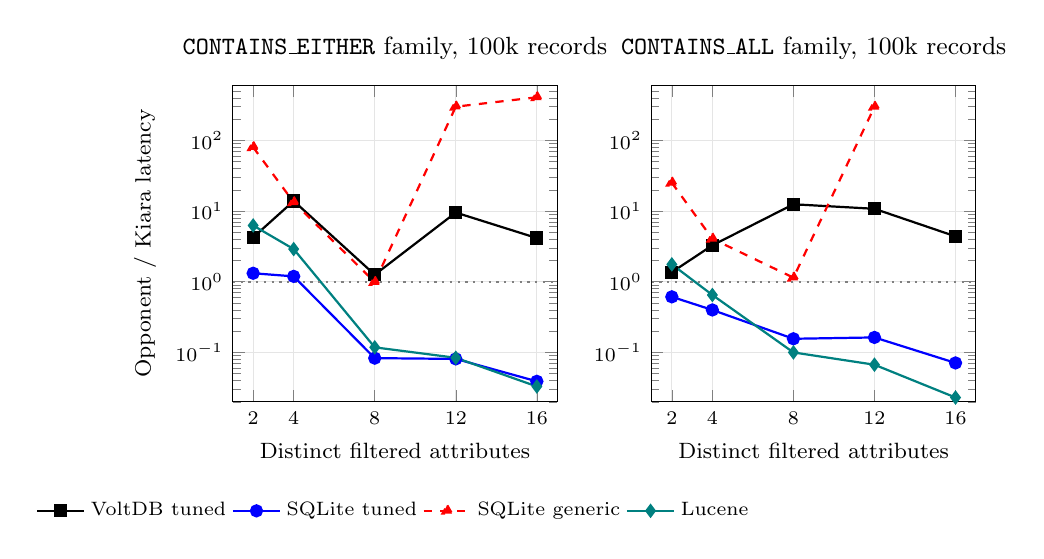
\begin{tikzpicture}
\begin{axis}[
  name=either, width=0.47\textwidth, height=5.6cm,
  ymode=log, ymin=0.02, ymax=600,
  xtick={2,4,8,12,16}, xmin=1, xmax=17,
  xlabel={Distinct filtered attributes}, ylabel={Opponent / Kiara latency},
  title={\small \op{CONTAINS\_EITHER} family, 100k records},
  tick label style={font=\scriptsize}, label style={font=\footnotesize},
  legend style={font=\scriptsize, at={(0.5,-0.28)}, anchor=north, legend columns=4, draw=none},
  grid=major, grid style={gray!20}]
\addplot[black, mark=square*, thick] coordinates {(2,4.246) (4,13.905) (8,1.257) (12,9.535) (16,4.151)};
\addplot[blue, mark=*, thick] coordinates {(2,1.319) (4,1.192) (8,0.083) (12,0.081) (16,0.039)};
\addplot[red, mark=triangle*, thick, dashed] coordinates {(2,80.115) (4,13.329) (8,0.990) (12,300.158) (16,407.571)};
\addplot[teal, mark=diamond*, thick] coordinates {(2,6.257) (4,2.898) (8,0.118) (12,0.084) (16,0.033)};
\addplot[gray, dotted, thick, forget plot] coordinates {(1,1) (17,1)};
\legend{VoltDB tuned, SQLite tuned, SQLite generic, Lucene}
\end{axis}
\begin{axis}[
  at={(either.east)}, anchor=west, xshift=12mm,
  width=0.47\textwidth, height=5.6cm,
  ymode=log, ymin=0.02, ymax=600,
  xtick={2,4,8,12,16}, xmin=1, xmax=17,
  xlabel={Distinct filtered attributes},
  title={\small \op{CONTAINS\_ALL} family, 100k records},
  tick label style={font=\scriptsize}, label style={font=\footnotesize},
  grid=major, grid style={gray!20}]
\addplot[black, mark=square*, thick] coordinates {(2,1.366) (4,3.275) (8,12.489) (12,10.773) (16,4.386)};
\addplot[blue, mark=*, thick] coordinates {(2,0.612) (4,0.399) (8,0.156) (12,0.163) (16,0.071)};
\addplot[red, mark=triangle*, thick, dashed] coordinates {(2,25.183) (4,4.058) (8,1.142) (12,298.414)};
\addplot[teal, mark=diamond*, thick] coordinates {(2,1.763) (4,0.650) (8,0.100) (12,0.067) (16,0.023)};
\addplot[gray, dotted, thick, forget plot] coordinates {(1,1) (17,1)};
\end{axis}
\end{tikzpicture}
\caption{Wide-filter results (S7) for 100,000 records: geometric-mean opponent/Kiara latency over three selectivity targets. Values above the dotted line favor Kiara. Generic-SQLite points at width 12 (both families) and width 16 (\op{CONTAINS\_EITHER}) are based on the one target that completed in every trial; the other targets exceeded the 60\,s deadline in every trial. Generic SQLite timed out on every \op{CONTAINS\_ALL} query at width 16, which therefore has no point. Kiara completed all queries.}
\label{fig:wide}
\end{figure*}

\subsection{Correctness Findings}
\label{sec:correctness}
The oracle uncovered four behaviors that a latency-only benchmark would have hidden.
\begin{enumerate}
\item \emph{Fractional truncation.} Because numeric keys are truncated to integers, \texttt{price < 0.20} returned none of 121 expected products, \texttt{price <= 19.50} also matched 19.99, and \texttt{price = 19.99} matched 209 products instead of 3 on the large catalog. Forty scenario--trial entries were excluded on this basis in each five-trial base suite (S3--S6).
\item \emph{Cross-attribute normalization.} The retail fixture indexes raw title tokens in one attribute and stemmed tokens in another. For the query \emph{lanterns}, Kiara returned 18 records, while Lucene and the oracle returned 20, including plural titles. Kiara keeps a single normalized form per keyword across all attributes the keyword binds to (Section~\ref{sec:text}). Keeping one form per bound attribute would correct this implementation limitation.
\item \emph{Interval comparator contract.} Version 2.0.15 failed to build the realistic schedule indexes. The defect was diagnosed and fixed in 2.0.16 (Section~\ref{sec:system}), and all builds subsequently succeeded.
\item \emph{Limits.} Different engines returned different valid subsets for limited queries. Applications that need deterministic pagination must impose an order.
\end{enumerate}

\section{Discussion}
\label{sec:discussion}

\subsection{When Is the Attribute Trie the Right Choice?}
The results support a precise rather than a universal claim. Kiara answers \emph{any} conjunction through one logical index per attribute. It is strongest when combinations are unpredictable, predicates involve collection membership or point-in-interval tests, and queries are moderately selective. Under those conditions it outperformed Lucene on every dataset, generic-index SQL configurations on 11 of 12 dataset entries, and even tuned VoltDB on every collection-family width in the wide-filter suite. Its text layer adds typo correction, stemming, prediction, and attribute-discovering keyword search over the same indexes, with no second engine to synchronize.

Conversely, when a few hot combinations are known in advance, a compound index serves them better. That is the case Proposition~\ref{prop:indexcount} excludes only when \emph{all} combinations must be served. The same holds for broad scalar windows, top-$k$ queries with limits, frequent rebuilds, tight memory budgets, and relevance-ranked text search. A practical consequence is that the approaches compose. An application can serve its few known hot combinations with dedicated access paths and route the long tail of ad hoc combinations to an attribute trie.

The preparation cost should be amortized explicitly. If a rebuild costs $\Delta B$ more than an alternative and saves $\Delta t$ per query, preparation pays off after $n^\ast=\Delta B/\Delta t$ queries per rebuild. On the 100,000-product catalog, for example, Kiara's additional build time over Lucene was about 178\,s. A workload saving 1\,ms per query would therefore need about 178,000 queries between rebuilds. The build-time remedy below would change this calculation substantially.

\subsection{Threats to Validity}
\emph{Internal validity.} All suites ran on a shared, virtualized host whose scheduling and thermal state were not controlled. VoltDB required JDK~11 while Kiara ran on JDK~21. The harness is a standalone measurement program rather than JMH. Five trials provide only exploratory intervals. Output representations differ: Java maps, Lucene stored fields, and \texttt{VoltTable} objects are not equal-cost encodings. Tuning used the evaluation fixtures, which favors the tuned opponents. The shared record class places a unique identifier at the first trie level. This layout is unfavorable to Kiara's build time and memory. It also removes nearly all prefix sharing, so it can change candidate sizes and therefore query costs. The experiments thus evaluate a largely degenerate trie layout rather than a schema ordered as the library documentation recommends.

\emph{External validity.} Catalog, schedule, and wide fixtures are synthetic, and the wide fixture uses mostly independent attributes. Real data with correlated attributes may benefit more from prefix sharing, or less. All measurements are single-threaded, warm, and in memory. We did not measure concurrent throughput, cold starts, durability, updates, or distributed operation.

\emph{Construct validity.} Equal-weight geometric means summarize ratios but do not represent any particular application's query mix. Sensitivity checks in the raw reports show that removing the most extreme query ratio can reverse a near-unity aggregate.

\emph{Conflict of interest.} The author created Kiara. To mitigate this, opponents received expert tuning while Kiara received none; correctness was enforced by an independent oracle; unfavorable results are reported prominently; and all raw data, plans, and harness code are published for independent replication.

\subsection{Limitations and Future Work}
\label{sec:future}
Each weakness identified in Section~\ref{sec:predictions} suggests a concrete remedy:
\begin{enumerate}
\item \emph{Linear-time loading (P6).} Keying trie children by hash map makes insertion $O(Nm)$ expected, as the TypeScript port already does.
\item \emph{Exact numeric keys.} Order-preserving encodings of IEEE-754 doubles, or scaled decimals, would remove fractional truncation without giving up ordered key arrays.
\item \emph{Fan-out-aware reduction (P2).} When a candidate collection's fan-out exceeds a threshold, merging its lists once, in $O(\|\mathcal{C}\|\log q)$, or representing it as a compressed bitmap~\cite{lemire2016roaring}, would remove the multiplicative factor in Eqs.~\eqref{eq:probeup}--\eqref{eq:expanddown}.
\item \emph{Selectivity-ordered evaluation and predicate fusion (P3, P4).} Ordering conditions by estimated candidate size, which is available exactly from posting-list lengths, and rewriting same-attribute comparisons into \op{BETWEEN} are both local changes.
\item \emph{Complement by difference.} Evaluating negations as a sorted-list difference against the positive side, rather than by enumerating keys, would bound \op{NOT\_EQUAL} and \op{NOT\_CONTAINS} by the size of the other operand.
\item \emph{Limit push-down (P5).} Lazily enumerating $\mathcal{R}$ in preorder would stop after $\lambda$ results.
\item \emph{Concurrency and updates.} The prepared structure is read-only, which suits lock-free concurrent readers. Atomic snapshot replacement provides updates. Neither has been characterized experimentally.
\item \emph{Text quality.} Keeping a normalized key per bound attribute would fix the cross-attribute normalization defect. Comparing value sets rather than counts would make minimum match exact. Levenshtein automata~\cite{schulz2002fast} for multi-edit correction, and term weighting within the winning coverage tier, would complement coverage-first semantics.
\item \emph{Explicit schema order.} Declaring level order through annotations or configuration, rather than relying on reflection order, would make trie layout portable. It would also let applications follow the high-cardinality-last guideline deliberately.
\end{enumerate}

\section{Conclusion}
\label{sec:conclusion}
Six years after the original description of equality search over depth-first-numbered attribute tries~\cite{kapoor2020efficient}, this paper presented the complete Kiara DB design. It covers typed, temporal, collection, and interval attributes; eleven operators; an adaptive structural join over disjunctive posting-list collections; and a text layer for correction, stemming, prediction, and attribute-discovering keyword search. We corrected the composite-index bound that motivates the design to $\binom{m}{\lfloor m/2\rfloor}$, derived a cost model in terms of candidate fan-out, and tested it in seven oracle-validated benchmark suites against Lucene, SQLite, and VoltDB. One logical index per attribute is competitive with, and often faster than, mature engines for ad hoc and collection-heavy conjunctions. Expert compound indexes remain superior for known scalar combinations and windows, and Kiara's current Java loader is its most significant practical weakness. The cost model identifies changes that address each observed weakness without abandoning the model.

\section*{Data Availability}
Kiara is open source~\cite{kiara2026software}. The benchmark harness, fixture generators, retail projection and its attribution, raw per-trial samples, native plans, index inventories, and generated reports are available in the Kiara demonstration repository~\cite{kiarademo2026benchmarks}.

\section*{Acknowledgment}
The author thanks the maintainers of Apache Lucene, SQLite, the Xerial JDBC driver, and VoltDB Community Edition. Generative AI tools (GitHub Copilot) assisted with benchmark-harness engineering, report drafting, and editing of this manuscript. The author reviewed, verified, and takes responsibility for all content, data, and conclusions.


\bibliographystyle{IEEEtran}
\bibliography{references}

\begin{IEEEbiographynophoto}{Anuj Kapoor}
is the founder of Kapoor Labs and the creator and maintainer of Kiara DB. His research interests include in-memory data structures, search, and query processing for read-mostly data. % TODO(author): add degrees, positions, and a photograph as required by IEEE Access.
\end{IEEEbiographynophoto}

\EOD

\end{document}
